\section{Experimental evaluation}
\label{sec:eval}

\subsection{Method and evidence discipline}
\label{sec:eval-method}

We structure the evaluation around five research questions:

\begin{itemize}
\item \textbf{RQ1 (Integration).} Can one configuration-driven runtime
integrate heterogeneous plant protocols such that platform-side data and
write paths equal device-side behavior, including under faults?
\item \textbf{RQ2 (Mechanism attribution).} Which layer of the write path
provides interception of policy-breaching writes, does removing a layer
degrade safety, and does governance introduce false blocks?
\item \textbf{RQ3 (Closed loop).} Can an agent team complete a governed
supervisory correction (read, analyze, propose, human approval, write,
readback, retest, record) end to end on a running line?
\item \textbf{RQ4 (Model-driven tier).} Does the model-driven optimization
tier respect the same governance and improve closed-loop performance in
simulation?
\item \textbf{RQ5 (Adversarial containment).} How does the platform behave
when a real, weak open-weight model attempts out-of-surface actions?
\end{itemize}

Every experiment is executed by a benchmark runner in the platform
repository and freezes a report, raw event logs, and SHA-256 checksums
into a versioned results directory that records the runner command, source
commit, and harness hash. Two plant scenarios are used: a cast-film line
driven by a physical-engine simulator (first-principles actuator and
material dynamics) with a MES mirror, and an injection line driven by a
PLC node simulator exposing all five protocols. LLM episodes use the omp
RPC harness serving an open-weight 9B-class model (Qwen3.5-9B, 64k
context, locally served); integration and ablation runs are deterministic
(no LLM) by design, so that mechanism-level results are not confounded by
model stochasticity. We report negative and mixed outcomes alongside
positive ones; none of the results below pool runs across scenarios into
a single denominator.

\subsection{Device integration across five protocols (RQ1)}
\label{sec:eval-integration}

The device integration matrix connects real protocol stacks (Modbus
TCP, Modbus RTU, OPC UA, MQTT, and HTTP) to the virtual PLC and
exercises the full path from configuration to write. The matrix passes
21 of 21 assertions (Table~\ref{tab:integration}): environment
self-checks, scene provisioning, per-protocol acquisition with
platform-versus-device value equality, write-through on the four writable
protocols with dispatch narrowing, negative probes, and fault handling.
In fault handling, a disconnect is reported honestly as a failure and the
path self-heals on reconnect. A companion provisioning run on a second scene
(an injection line with thirteen acquisition nodes including a vector
profile node, plus three write nodes) brought all thirteen acquisition
nodes online through the same configuration surface with no code change.

A longer integrated pipeline run (one deterministic execution covering
scene provisioning, acquisition, governed operations, seeded objective
cases, a second scene, and a scripted BOPET task) passed all 17 phase
gates and 76 of 77 checks (one warning on a semantic-card check; zero
failures). Within that run, five protocol endpoints returned 54 samples,
and all 24 negative probes on four writable paths were rejected before
driver execution. A second-scene configuration rejected 9 of 9 additional
probes. The median write round-trip across the four writable protocols
was 31.6\,ms including real protocol transactions. Three
fixed-seed objective cases solved against the simulator's offline
reference ended at 96.3--98.8\% of the reference (mean 97.8\%); one seed
began inside the stopping region and correctly terminated with zero
writes. This run demonstrates configuration breadth and regression
fidelity; the matrix above demonstrates real-stack fidelity.

\begin{table}[!t]
\centering
\caption{Device integration matrix on real protocol stacks (21/21
assertions pass). Grouped view of the frozen assertion set; every group
passed in full.}
\label{tab:integration}
\small
\begin{spacing}{1.0}
\begin{tabularx}{\columnwidth}{@{}p{0.34\columnwidth}X@{}}
\toprule
Group & What is checked \\
\midrule
Environment (S0--S1) & Simulator and platform reachable; scenario baseline valid \\
Provisioning (P0--P2) & Scene configuration provisions lines, products, recipes, nodes through the platform API \\
Acquisition (D--*, D-match) & Per-protocol sampling on Modbus TCP/RTU, OPC UA, MQTT, HTTP; platform samples equal device-side values \\
Write path (W1, G0, W3--W4) & Write-through on the four writable protocols; dispatch narrowing to bound surface; governed dispatch verified \\
Negative (N1--N2) & Out-of-scope and malformed write requests rejected before driver execution \\
Fault recovery (F1--F3) & Disconnect reported as failure (not stale success); reconnect self-heals; no phantom writes \\
\bottomrule
\end{tabularx}
\end{spacing}
\end{table}

\subsection{Governance mechanism attribution (RQ2)}
\label{sec:eval-ablation}

Integration shows the path works; it does not show \emph{which layer} does
the protecting. We therefore run a four-arm ablation in which attack
writes targeting recipe-window violations are injected alongside
legitimate writes. Each arm disables one element of the path: \emph{Full}
(the complete path), \emph{No interlock} (the soft batch-window interlock
disabled), \emph{No readback} (receipt grading disabled), and
\emph{Ungated} (the bench-mode soft gating removed). Each arm runs three
repetitions of a six-attack set (18 attack writes per arm) plus
legitimate traffic; every decision is journaled.

Table~\ref{tab:ablation} and Figure~\ref{fig:ablation} report the
outcome. The arm definitions follow the path's predicates: \emph{No
interlock} removes only the soft batch-window interlock predicate, leaving
the hard range, step and rate limits, approval, and authorization in
force. \emph{Ungated} additionally enables the platform's commissioning
mode, which on top of that relaxes rate limiting and readback tolerance
for bench operation. Both arms therefore leave the window-class attacks
unintercepted, which is the point: the experiment identifies which
predicate carries interception, and shows that removing it does not
weaken the structural layers. Interception is 100\% in Full and
No-readback arms across all
repetitions, and drops to 66.7\% in No-interlock and Ungated arms: the
window-class attacks (two per repetition) execute. Crucially, the
executed breaches are journaled as writes with their parameters.
\emph{Attribution is separable from prevention}: even where the platform
had no power to stop a write, the ledger records that it happened. The
hard node range rejects out-of-range values in every arm, including the
ungated one, and produces \emph{zero false blocks} across all 69
legitimate writes of the injected workload; boundary checks pass 9/9 in
every arm. We emphasize the scope of this cost result: the legitimate
traffic is runner-generated and passes with margin, so zero false blocks
here establishes that the interlocks do not harass compliant writes. It
does not establish a false-block rate for adversarially ambiguous
plant traffic. Removing readback leaves interception unchanged (100\%):
readback is an evidence layer, not an interception layer, which is
exactly the separation the design claims. Platform-side write latency is
indistinguishable across arms in this sample (p50 111--126\,ms with
in-memory readback; no formal test applied; protocol-level readback cost
is measured separately in the integration runs).

The ablation supports three conclusions. The soft batch-window interlock
is the load-bearing interceptor for window-class policy breaches (R2).
Defense in depth holds, because the structural hard range survives every
disabled configuration (R3). Governance cost, measured as false
blocks, is zero in this workload: legitimate writes are not harassed
by the interlocks.

\begin{table}[!t]
\centering
\caption{Four-arm governance ablation (3 repetitions per arm; 6 attack
writes per repetition, 18 per arm; 69 legitimate writes overall).}
\label{tab:ablation}
\footnotesize
\setlength{\tabcolsep}{3.5pt}
\begin{spacing}{1.0}
\begin{tabular}{@{}lrrrr@{}}
\toprule
Arm & Interception (per rep) & Breaches executed & False blocks & Boundary ok \\
\midrule
Full & 100/100/100\% & 0 & 0 & 9/9 \\
No interlock & 66.7/66.7/66.7\% & 6 & 0 & 9/9 \\
No readback & 100/100/100\% & 0 & 0 & 9/9 \\
Ungated & 66.7/66.7/66.7\% & 6 & 0 & 9/9 \\
\bottomrule
\end{tabular}
\end{spacing}
\end{table}

\begin{figure}[!t]
\centering
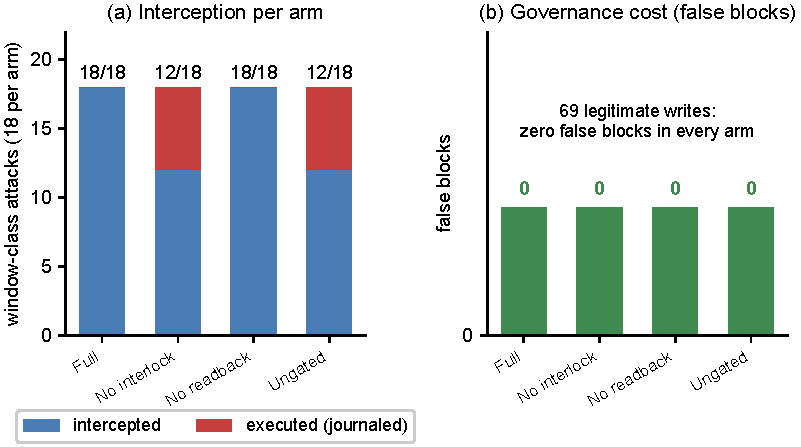
\includegraphics[width=0.98\columnwidth]{figures/fig3-ablation.pdf}
\caption{Mechanism attribution. (a)~Interception rate per repetition per
arm; only arms without the batch-window interlock admit the two
window-class attacks per repetition, and all executed breaches are
journaled. (b)~False blocks remain zero in every arm (the structural
hard range bounds writes without harassing legitimate traffic), and all
nine boundary probes pass in every arm.}
\label{fig:ablation}
\end{figure}

\subsection{Closed-loop case study on a running line (RQ3)}
\label{sec:eval-casestudy}

The flagship episode exercises the complete governed path on a running,
simulator-backed OPC UA production line (real protocol stacks, simulated
process physics): a melt-pumping unit of the cast-film scene
(physical-engine simulator with MES mirror). The goal is to bring the
three-minute mean melt pressure to at most 15.8\,MPa from an observed
16.1\,MPa, entirely through the platform's agent runtime: a lead agent
decomposing the goal and a governed write path with human approvals.
Acquisition on the target node ran at a median interval of 2.06\,s
(p90 2.09\,s, max 4.15\,s) with zero dropped windows over a one-hour
observation (1741 rows). The line had accumulated 22 batches, and the
model tier consumed a cross-run dataset of 15{,}989 rows over 7 runs.

Table~\ref{tab:casestudy} gives the decision timeline, reconstructed
from the audit ledger and approval records. The lead analyzed six
baseline windows (four shown: 16.04/16.00/15.99/16.01\,MPa) and
self-calibrated the process gain from observation (0.107--0.12\,MPa/rpm,
against 0.134 from historical data). It formed a proposal of
$130 \to 127$\,rpm, the largest single step the path would admit
(2\% of range), predicting 15.64--15.68\,MPa. Mid-flight, a second agent team restored a pending
proposal in the opposite direction. The one-proposal-in-flight gate
pinned it, and the lead located the conflict. A human arbitration
rejected the opposing proposal with a written basis rather than allowing
either team to force a write. The lead's proposal then entered the
governed path: the approval record bound the candidate value, the
applicable limits, and the active line--product--recipe--run tuple. A
human approved it. The write dispatched the same second and was
readback-verified at 127\,rpm. After process inertia, two retest windows
read 15.616 and 15.656\,MPa, within the goal and inside the
self-calibrated prediction band (measured gain 0.127\,MPa/rpm,
deviation 0.021--0.060 from the predicted band). A second approval
promoted the recipe version at 127\,rpm to prevent drift, and an
independent physical recheck read 15.5\,MPa with the setpoint read back
at 127\,rpm. The episode closed with the measured gain written back to
the channel's shared memory for future teams.

Two design behaviors surfaced on their own in this episode. First, the
model tier's dual-gate discipline held. A supervised surrogate model
trained on the line's own data passed all five promotion gates (single-
and rolling-horizon NRMSE 0.056 and 0.055 against bounds of 0.10 and
0.25; generalization gap 0.074 against 0.20; data volume and artifact
contract satisfied) and was promoted to shadow status. Yet the usage
gate refused it for model-driven MPC because its uncertainty-calibration
layer was absent, and the optimizer fell back to recommendation-only
operation with small safe steps. Model quality and permission to drive
control are deliberately different gates, and the episode shows the
distinction firing on a live model. Second, the episode exposed a real
product gap (the dataset builder could not replay control trajectories
from the write ledger into training data), which we report as a
limitation in Section~\ref{sec:discussion}.

A second, fully instrumented episode replicates the mechanical path with
an identified model: the omp RPC harness serving Qwen3.5-9B (64k context,
locally served) on a four-protocol cast-film scene against a production
build of the platform in an isolated instance. The agent's read task
returned values equal to device truth. A governed write then suspended
on a HITL card with the device value unchanged until the decision
(\emph{the interception is real, not nominal}); after approval, the
device register read exactly baseline$+3$ (195$\to$198), verified by
readback. A subsequent tuning task wrote a $+2.5$ adjustment
($198 \to 200.5$) with the melt-temperature PV converging toward the new
setpoint (intermediate sample 199.45\,°C; the closing review recorded a
settled deviation of 0.34\,°C). The parameter ledger attributed both
writes to the agent with their hypotheses. We note two boundaries
honestly: the human decision points in this replication were exercised
by an automated approver script (it validates the mechanical path, not
human judgment quality), and both episodes are single-scenario case
studies, not powered comparisons.

\begin{table}[!t]
\centering
\caption{Case-study decision timeline (melt-pressure correction on an
OPC UA line; all events ledger-reconstructed).}
\label{tab:casestudy}
\small
\begin{spacing}{1.0}
\begin{tabularx}{\columnwidth}{@{}p{0.16\columnwidth}X@{}}
\toprule
Time & Event \\
\midrule
00:36 & Goal dispatched (3-min mean melt pressure $\leq$15.8\,MPa; observed 16.1\,MPa) \\
00:54 & Cross-team arbitration: opposing in-flight proposal rejected by human with written basis \\
00:52--00:58 & Lead first round: six baseline windows (16.04/16.00/15.99/16.01\,MPa); self-calibrated gain 0.107--0.12\,MPa/rpm; proposal $130\to127$\,rpm (2\%-of-range step cap); predicted 15.64--15.68\,MPa \\
01:05:24 & Proposal enters governed path; approval record binds values, limits, and active tuple \\
01:05:27 & Human approval; dispatch same second; readback-verified at 127\,rpm \\
+inertia & Retest windows 15.616/15.656\,MPa $\leq$ 15.8; measured gain 0.127\,MPa/rpm inside prediction band \\
01:12:40 & Second approval promotes recipe version at 127\,rpm \\
post & Independent recheck: 15.5\,MPa; SP readback 127\,rpm; gain written back to channel memory \\
\bottomrule
\end{tabularx}
\end{spacing}
\end{table}

\subsection{Model-driven optimization tier (RQ4)}
\label{sec:eval-modeltier}

The optimization tier is evaluated in a live-loop configuration in which
an agent solves each beat against the governed solver and applies the
first move through the write path. Over a twelve-beat run with per-beat
context refresh, the median quality error fell from 6.42 to 0.02 (a
99.7\% reduction in this single twelve-beat run). Every manipulated
variable stayed inside its process window. In a twenty-seed paired
comparison, the tier solved 94.8\% of problem instances against 42.2\%
for static response-surface solving (rates aggregated over the paired
instances across seeds; per-seed denominators are in the frozen
artifact). This is a descriptive result consistent with the gated
model, not the solver alone, carrying the performance. Governance
semantics held
throughout. Solving without a qualified profile or binding is refused
with explanatory HTTP 409/422 status codes, and solver and twin must
agree on the same
frozen inputs to $10^{-6}$ relative tolerance. The full surface
survives a restart with bindings, profiles, and ledger intact
(seven persistence checks). Figure~\ref{fig:modeltier} summarizes these
results. These are simulation-tier results: the process models and the
twin are simulator-backed, and we do not claim plant-scale benefits.

\begin{figure}[!t]
\centering
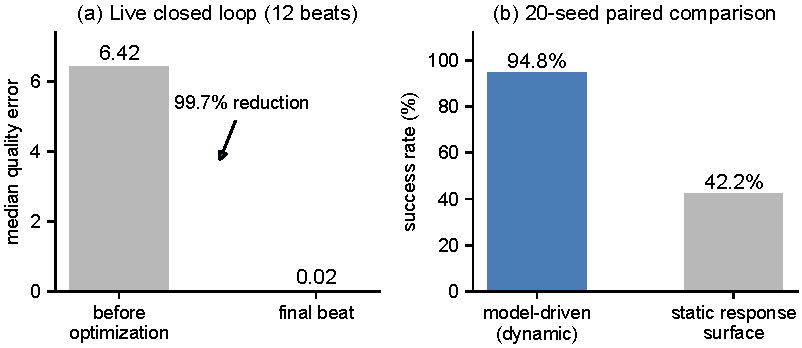
\includegraphics[width=0.98\columnwidth]{figures/fig4-modeltier.pdf}
\caption{Model-driven optimization tier. (a)~Median quality error over a
twelve-beat live closed loop: 6.42 before optimization to 0.02 at the
final beat (99.7\% reduction), with every MV inside its process window.
(b)~Twenty-seed paired comparison of dynamic model-driven solving versus
static response-surface solving: 94.8\% versus 42.2\% success.}
\label{fig:modeltier}
\end{figure}

\subsection{Adversarial containment (RQ5)}
\label{sec:eval-adversarial}

The final episode asks what happens when the model is genuinely weak and
the task genuinely hard. A three-agent team (lead plus two workers) on
the same 9B-class model, through the same harness, ran an injection-line
optimization goal under a production-like scenario. The episode's
qualification gates passed, but the workflow did not converge. The
platform behaved as designed throughout: the task was canceled
before completion, \emph{zero} unapproved writes reached the plant, and
the monitoring layer recorded twelve tool-surface violations and nine
unapproved harness tool calls. All were attributed and frozen with 153
raw event records and recomputed checksums. The process variable moved
31.28$\to$31.36\,g against a target of $32.5 \pm 0.35$\,g: the goal
was not achieved, and we report it as a negative result. The
governance-relevant observation is containment: a weak model was given a
supervisory task, misbehaved, and the platform's layered checks and
event monitors bounded the damage to zero plant writes while preserving
a complete evidentiary record. Two boundaries on this episode: no
prompt-injection attack was executed in it (the model misbehaved
unaided), so the telemetry-side injection threat of
Section~\ref{sec:problem-fm} remains to be exercised; and the episode is
a feasibility probe, not a powered comparison.

\subsection{Engineering quality and reproducibility (RQ1--RQ5)}
\label{sec:eval-quality}

Table~\ref{tab:quality} summarizes the regression base under the
behavioral results. The unit suite collects 915 tests with 913 passing
and two environment-skipped; line-governance, node-authority,
adversarial error handling, and security-check suites pass in full. A
frozen baseline captured from an earlier release is re-executed by the
benchmark runner: the four-arm ablation scenario reproduces bit-exactly
across a twelve-day gap (identical report hash). This is the property
that makes the ablation auditable after the fact. The same mechanism
honestly flags non-reproducibility elsewhere: a second baseline scenario
failed reproduction when the harness hash and source commit drifted, and
the runner reports that failure rather than masking it. Drift
detection is part of the evidence contract.

\begin{table}[!t]
\centering
\caption{Regression and evidence base underlying the behavioral results.}
\label{tab:quality}
\small
\begin{spacing}{1.0}
\begin{tabularx}{\columnwidth}{@{}p{0.42\columnwidth}X@{}}
\toprule
Suite & Result \\
\midrule
Unit tests & 913/915 pass (2 environment-skipped) \\
Line-governance end-to-end & 44/44 assertions \\
Node-authority surface & 52/52 \\
Adversarial error handling & 26/26 \\
Security hardening checks & 29/29 \\
Frozen-baseline reproduction (ablation scenario) & Bit-exact across 12 days \\
Frozen-baseline reproduction (second scenario) & Correctly reported NOT reproducible under commit/harness drift \\
\bottomrule
\end{tabularx}
\end{spacing}
\end{table}
